% Prof. Dr. Ausberto S. Castro Vera
% UENF - CCT - LCMAT - Curso de Ci\^{e}ncia da Computa\c{c}\~{a}o
% Campos, RJ,  2019
% Disciplina: An\'{a}lise e Projeto de Sistemas
% Aluno: Luis Fernando Peixoto Cabral


\chapterimage{sistemas.png} % Table of contents heading image
\chapter{ Introdu\c{c}\~{a}o}


O sistema a ser desenvolvido nos decorreres dos capítulos é pensado em um hospital, onde      será apresentados passo a passo desde a etapa de planejamento, analise até a etapa de projeto.O Trabalho tem como referencial teórico o livro \cite{Dennis2014}.
Neste capitulo será feita uma descrição do projeto a ser desenvolvido. 



 \section{Descri\c{c}\~{a}o do Sistema Computacional a desenvolver}

O sistema terá dois pilares prioritários um deles, é facilitar a comunicação entre os setores do hospital, na qual irar permitir o setor administrativo gerenciar as informações, permitindo tomadas de decisões mais eficazes. O segundo Pilar é oferecer ao paciente diferentes formas de atendimento, por aplicativo, site, ligação telefônica e diretamente no próprio hospital \\

\textbf{Aplicativos e website} 

Um dos principais objetivos do projeto, é oferecer recursos para os pacientes, na qual possa proporcionar uma boa experiência com o sistema. Será possível através do aplicativo e website, realizar agendamento de consultas e exames, verificar resultados de exames, ter acesso a boletim médico de parentes que estão na UTI, realização de pagamentos e por fim será possível sanar dúvidas de forma online com um médico de plantão. \\


\textbf{Monitoramento de socorro} 

O sistema oferecerá suporte ao paciente durante a espera da chegada do pronto-socorro, onde o paciente por meio do aplicativo ou website, efetuará a solicitação  de socorro e imediatamente por meio de uma chamada de vídeo irá ser possível receber orientações de um médico de plantão, além de mostrar o trajeto da ambulância com o tempo de estimativa de chegada ao local. \\

\begin{figure}[H]
              \begin{center}
                  \caption{Sistema de pronto-socorro} \label{afp}
                  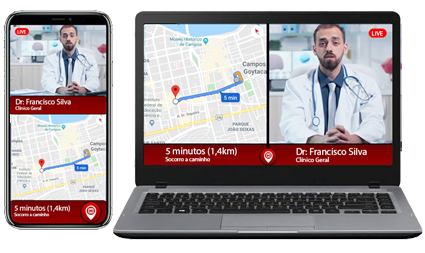
\includegraphics[width=15cm]{Pictures/smartENotoe.png} \\
                    {\tiny \sf Fonte:o autor }

              \end{center}
             \end{figure}


\textbf{Controle de estoque} 

O setor de farmácia do hospital terá o recurso de controle de estoque, onde terá como objetivo facilitar o trabalho dos funcionários e evitar possíveis desperdícios. O sistema também tera como função, notificar quando um determinado medicamento esta próximo da data de validade, e também sera possível solicitar medicamentos com o fornecedor através do sistema. \\

\textbf{Sistema de Gestão} 

O sistema irá proporcionar ao setor administrativo o melhor planejamento estratégico e a fiscalização de todos os setores do hospital. Será possível emitir relatórios financeiros de todos setores, proporcionando assim a avaliação da condição financeira do hospital. O sistema também contará com as funções de: emissão de notas fiscais , emissão de recibos, controle de fluxo de caixa, controle de plano de contas e centro de custos. E também irá gerar os relatórios de cadastro de paciente e fornecedores. Através de todos esses recursos, será possível proporcionar maior facilidade em gerenciar recursos do hospital, pelo setor administrativo. \\


\textbf{Sistema médico} 

Através do sistema, será possível proporcionar aos médicos uma melhor organização no trabalho. Através das funções de: gerenciar e verificar plantões e gerenciar consultas. Também será possível adicionar boletins médicos no sistema, onde o paciente poderá consultar, através do aplicativo ou website. O médico também poderá realizar a seguintes funções no sistema: o encaminhamento do paciente para realização de exames e por fim será possível receitar medicamentos pelo próprio sistema, onde o paciente poderá imprimir a receita. Através desses recursos irá proporcionar uma melhor experiência ao paciente e ao médico, em relação ao sistema.
 
 
  \section{Descrição dos subsistemas}
  O sistema será composto por 5 subsistema, na qual cada subsistema será destinado para um setor do hospital.
        \subsection{Sistema administrativo}
 O sistema administrativo deve permitir ter acesso a todas informações dos setores do hospital, para que possa ser um meio adequado de administrar e gerenciar os recursos, facilitando assim o poder de tomar decisões rápidas e eficientes no dia a dia.

        \subsection{Sistema de atendimento}
O Setor de atendimento é responsável pela marcação de consultas e exames. Tem   responsabilidade também de atender os chamados de emergências, na qual é imediatamente encaminhado para o sistema de pronto-socorro. Os atendimentos também devem ser feitos via aplicativo, via site, via ligação telefonica e diretamente na recepção do hospital. O sistema terá a função de se trabalhar com horários marcados, sendo assim o paciente irá ao hospital apenas no horário combinado, eliminando assim as filas de espera.
        \subsection{Sistema de farmácia}
Através do sistema, o médico responsável pelo paciente prescreve o medicamento, restando o paciente pegar na própria farmácia do hospital.
O sistema deve ter um controle de estoque para os medicamentos, para que quando necessário, através do próprio sistema seja feita a solicitação ao setor administrativo a reposição de um determinado medicamento.


        \subsection{Sistema de Pronto-Socorro}
Após a solicitação de emergência feita pelo setor de atendimento, o sistema tem a função de repassar a solicitação para a ambulância e através de um gps o sistema deve calcular a rota do chamado.
        \subsection{Sistema de RH}
O sistema permiti ter uma visão geral de todos os funcionários do hospital
 \section{Identificando as componentes do meu sistema}
A seguir será apresentado os equipamentos essenciais para o funcionamento do sistema, além de mostrar como será feito a logística de treinamento para os funcionários que usufruirão do novo sistema.
     \subsection{Componente: Hardware}

\begin{itemize}
\item \textbf{Monitores}
  \subitem -  para o setor médico
  \subitem - para o setor administrativo
  \subitem -  para o setor de atendimento
  \subitem -  para o setor de RH
  \subitem -  para o setor de Pronto-Socorro
  \item \textbf{ Microcomputadores processador 3.0Ghz, HD de 500Gb e 4Gb de memória Ram}
  \subitem -  para o setor médico
  \subitem -  para o setor administrativo
  \subitem -  para o setor de atendimento
  \subitem -  para o setor de RH
  \subitem -  para o setor de Pronto-Socorro
  \item  \textbf{Impressoras}
   \subitem - para o setor médico
    \item  \textbf{Impressoras multifuncional}
  \subitem -  para o setor administrativo
  \subitem -  para o setor de atendimento
  \subitem -  para o setor de RH
  \item  \textbf{Smart TV de 40 polegadas}
    \subitem para o setor de Pronto-Socorro
  \item  \textbf{GPS}
  \item \textbf{ Roteador Wireless}
  \item  \textbf{Servidor}
  \item  \textbf{switchs}

\end{itemize}



     \subsection{Componente: Software}
\begin{itemize}
\item Sistema
  \subitem - Sistema Administrativo
  \subsubitem * Gerenciamento de Finanças
  \subitem - Sistema Medico
  \subsubitem * Gerenciamento de pacientes
  \subitem - Sistema de farmácia
  \subsubitem * Controle de estoque
  \subitem - Sistema de RH
  \subsubitem * Gerenciamento de Funcionários
   \subitem - Sistema de Pronto-Socorro
  \subsubitem * Software de gerador de rota

  \item Sistemas operacionais proprietário
  \item Pacotes Office


\end{itemize}


     \subsection{Componente: Pessoas}


\begin{itemize}
\item Programadores
\item Analista de Sistema
\item Chefe do Projeto
\item Arquitetos de software
\item Projetista
\item Avaliadores de Qualidade
  \item   Médicos
  \item  Funcionários  da administração
  \item   Atendentes
  \item  Socorrista
  \item   Funcionários  do RH
  \item Funcionários de manutenção
  \item Pacientes
  \end{itemize}



     \subsection{Componente: Banco de Dados}
\begin{itemize}

  \item Pacientes
  \item Finanças
  \item Funcionarios
  \item Resultado de Exames
  \item Estoque de medicamento
  \end{itemize}


     \subsection{Componente: Documentos }
  \begin{itemize}
  \item Relatórios
  \item Resultados de exames
  \item Atestado medico
  \item Prontuário médico
  \item Notas fiscais
   \item Manuais do sistema
  \item Diagramas UML
  \item Orçamentos
\end{itemize}

     \subsection{Componente: Metodologias ou Procedimentos}
\begin{itemize}
\item \textbf{Levantamento de requisitos}
  \subitem -Listagem de todos os equipamentos que serão necessários para o funcionamento do sistema

 \item\textbf{ Analise}
  \subitem -Construção do modelo de representação do desenvolvimento do sistema
   \subitem -Estudo da interação dos componentes com o sistema
    \subitem  -Estudo detalhado dos requisitos

  \item \textbf{Implementação}
  \subitem -Codificação
   \subitem -Criação de aplicativo e website
    \subitem  -Criação do Banco de Dados
     \subitem -Montagem do servidor
   \item \textbf{Testes}
  \subitem -Atividade de teste para verificação de falhas no sistema
   \subitem -Verificação de segurança

    \item \textbf{Treinamento dos Funcionários}
  \subitem -O treinamento será realizado por setores do hospital
   \subitem -Os Setores de RH e administrativo terão uma única aula sobre o sistema, em dias diferentes com todos os funcionários de um determinado setor.
   \subitem -O treinamento dos setores de Atendimento, Medico e de Pronto-socorro, ocorrerão individualmente com cada funcionário em um horário de folga.

   \item \textbf{Implantação}
  \subitem -Sistema colocado no Ambiente de usuário
   \subitem -Manual do sistema realizado
  \subitem -Realização da importação dos dados
   \subitem -A implantação do sistema deverá ser feita em gradualmente sem atrapalhar o funcionamento do hospital
  \end{itemize}
     \subsection{Componente: Mobilidade}
 \begin{itemize}
 \item Smartphones para Funcionários
   \item Ligação telefônica
  \item Website
  \item Aplicativo
  \end{itemize}

     \subsection{Componente: Nuvem}
 \begin{itemize}
 \item Backup de dados via nuvem
   \item Hospedagem
  \subitem -Website
  \subitem -Aplicativo

\end{itemize}

